%!TEX root = ../diss.tex
\tikzstyle{element}=[rectangle, thick,
                     inner sep=0.1cm, rounded corners]
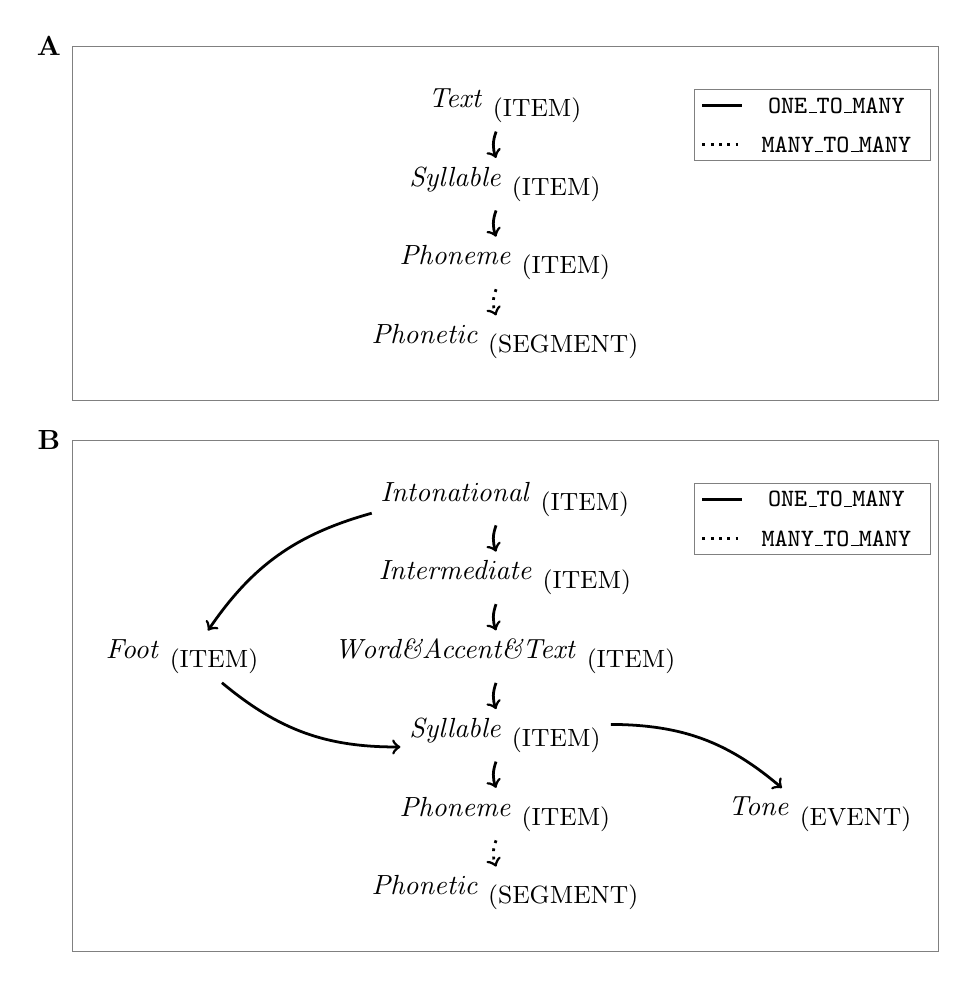
\begin{tikzpicture}
  
  %%%%%%%%%%%%%%%%%%%%%%%%%%%%%%
  %%%%%%%%%%%%%%%%%%%%%%%%%%%%%%
  % hierarchy

  %%%%%%%%%%%%%%%%%%%%%%%%%%%%%%
  % nodes
  % simple
  \draw[gray] (-5.5, 9.75) rectangle (5.5, 5.25);
  \node (a) at (-5.8, 9.75){\textbf{A}};

  \node (text) at (0, 9) [element] {\textit{Text} \textsubscript{\small{(ITEM)}}};

  \node (syl) at (0, 8) [element] {\textit{Syllable} \textsubscript{\small{(ITEM)}}};
  
  \node (phoneme) at (0, 7) [element] {\textit{Phoneme} \textsubscript{\small{(ITEM)}}};
  
  \node (phonetic) at (0, 6) [element] {\textit{Phonetic} \textsubscript{\small{(SEGMENT)}}};

  % complex
  \draw[gray] (-5.5, 4.75) rectangle (5.5, -1.75);
  \node (b) at (-5.8, 4.75){\textbf{B}};

  \node (into_c) at (0, 4) [element] {\textit{Intonational} \textsubscript{\small{(ITEM)}}};

  \node (interm_c) at (0, 3) [element] {\textit{Intermediate} \textsubscript{\small{(ITEM)}}};

  \node (word_c) at (0, 2) [element] {\textit{Word\&Accent\&Text} \textsubscript{\small{(ITEM)}}};

  \node (foot_c) at (-4.1, 2) [element] {\textit{Foot} \textsubscript{\small{(ITEM)}}};


  \node (syl_c) at (0, 1) [element] {\textit{Syllable} \textsubscript{\small{(ITEM)}}};
  
  \node (phoneme_c) at (0, 0) [element] {\textit{Phoneme} \textsubscript{\small{(ITEM)}}};

  \node (tone_c) at (4, 0) [element] {\textit{Tone} \textsubscript{\small{(EVENT)}}};
  
  \node (phonetic_c) at (0, -1) [element] {\textit{Phonetic} \textsubscript{\small{(SEGMENT)}}};

  %%%%%%%%%%%%%%%%%%%%%%%%%%%%%%
  % legends
  % simple
  \draw[gray] (2.4, 9.2) rectangle (5.4, 8.3);
  \node (leg_simp_o2m) at (4.2, 9) [element] {\small{\texttt{ONE\_TO\_MANY}}};
  \node (leg_sim_m2m) at (4.2, 8.5) [element] {\small{\texttt{MANY\_TO\_MANY}}};
  \draw [-, line width=1] (2.5, 9) to (3.0, 9);
  \draw [-, line width=1, dotted] (2.5, 8.5) to (3.0, 8.5);

  % complex
  \draw[gray] (2.4, 4.2) rectangle (5.4, 3.3);
  \node (leg_simp_o2m) at (4.2, 4) [element] {\small{\texttt{ONE\_TO\_MANY}}};
  \node (leg_sim_m2m) at (4.2, 3.5) [element] {\small{\texttt{MANY\_TO\_MANY}}};
  \draw [-, line width=1] (2.5, 4) to (3.0, 4);
  \draw [-, line width=1, dotted] (2.5, 3.5) to (3.0, 3.5);

  %%%%%%%%%%%%%%%%%%%%%%%%%%%%%%
  % links
  % simple
  \draw [->, line width=1] (text) to [bend right=20] (syl);

  \draw [->, line width=1] (syl) to [bend right=20] (phoneme);

  \draw [->, line width=1, dotted] (phoneme) to [bend right=20] (phonetic);

  % complex
  \draw [->, line width=1] (into_c) to [bend right=20] (interm_c);

  \draw [->, line width=1] (into_c) to [bend right=20] (foot_c);

  \draw [->, line width=1] (interm_c) to [bend right=20] (word_c);

  \draw [->, line width=1] (word_c) to [bend right=20] (syl_c);

  \draw [->, line width=1] (foot_c) to [bend right=20] (syl_c);

  \draw [->, line width=1] (syl_c) to [bend right=20] (phoneme_c);

  \draw [->, line width=1] (syl_c) to [bend left=20] (tone_c);

  \draw [->, line width=1, dotted] (phoneme_c) to [bend right=20] (phonetic_c);

  
\end{tikzpicture}
